\documentclass{beamer}
\usepackage[british]{babel}
\usepackage[utf8]{inputenc} % This package will support Turkish chars

% Some useful packages I use frequently
\usepackage{hyperref}
\usepackage{stmaryrd}
\usepackage{color}
\usepackage{amsmath,amssymb}
\usepackage{graphicx}

% vertical separator macro
\newcommand{\vsep}{
  \column{0.0\textwidth}
    
\begin{tikzpicture}
      \draw[very thick,black!10] (0,0) -- (0,7.3);
    \end{tikzpicture}
}

% Beamer theme
\usetheme{Bilkent}
\usefonttheme[onlysmall]{structurebold}
\mode<presentation>
\setbeamercovered{transparent=10}

% align spacing
\setlength{\jot}{0pt}

%\setbeamertemplate{navigation symbols}{}%remove navigation symbols

\title{Investigating the Validity of Ground Truth in Code Reviewer Recommendation Studies}
\author[]{\textbf{Emre Doğan}, Eray Tüzün, K. Ayberk Tecimer, H. Altay Güvenir}
\institute{MSc Student \newline Computer Engineering Department \newline Bilkent University}
\date
    {ESEM 2019\\
    Porto de Galinhas, Brazil \\
    \today}

\begin{document}

% Insert Titlepage before starting content.
\begin{frame}
  \titlepage
\end{frame}

% Insert table of contents if necessary
\begin{frame}
  \frametitle{Outline}

  \tableofcontents
\end{frame}


% Insert slides below.
\section{Introduction}

\subsection{Code Review and Code Reviewer}

\begin{frame}{\large What is Code Review, Who is a Code Reviewer?}

  \textbf{Code Review:} A systematic examination of source code in order to highlight bugs and enhance the code quality.
  \newline \newline
  \textbf{Code Reviewer:} The developer performing a code review.
  \begin{figure}
    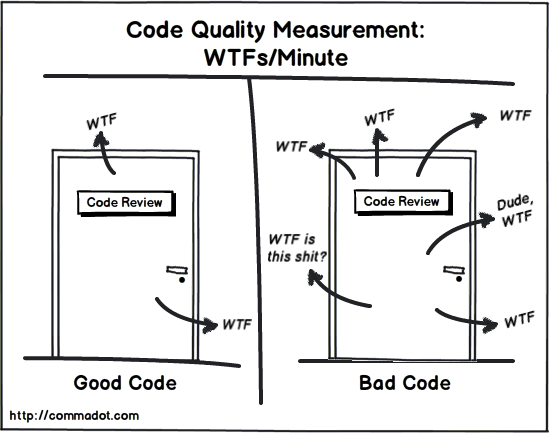
\includegraphics[scale=0.3]{img/code_review_wtf.png}
    %\caption{lion!!}
    \end{figure}
    
  %\begin{itemize}
  %    \item Using math equations
  %    \item Referencing Tables and Figures, as well as citations \cite{buyukccakir2018novel}
  %\end{itemize}
  
\end{frame}

\subsection{Code Reviewer Recommendation}

\begin{frame}
\frametitle{How to find an efficient code reviewer?}

    %\begin{block}{Fact:}
    %\begin{itemize}
    %\item Code reviewing is not the most fun activity for a developer.
    %\item But it is a crucial step of software quality assurance process.
    %\end{itemize}
    %\end{block}
    %\pause
    \begin{itemize}
    \item Code reviewer recommendation models/tools help us to choose efficient reviewers.
    \item These tools help software teams:
        \begin{itemize}
            \item to find reviewers who can find more(critical) bugs in the source code.
            \item to speed up the code review process.
        \end{itemize}
  \end{itemize}


\end{frame}




\subsection{How Reviewers are Selected}

\begin{frame}
\frametitle{\large Reviewer Selection in Recommendation Models }

  \begin{figure}
    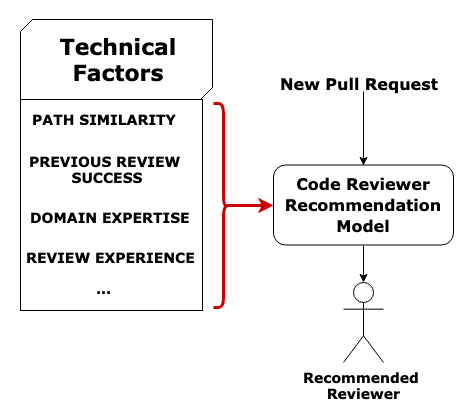
\includegraphics[scale=0.5]{img/algos.png}
    \end{figure}

\end{frame}

\begin{frame}
\frametitle{\large Reviewer Selection in Real Life }

  \begin{figure}
    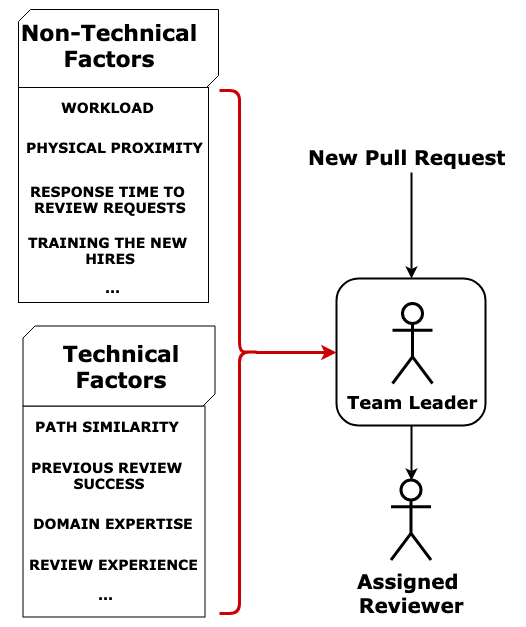
\includegraphics[scale=0.47]{img/real-life.png}
    \end{figure}

\end{frame}

\begin{frame}
\frametitle{\large Reviewer Selection in Real Life }

  \begin{figure}
    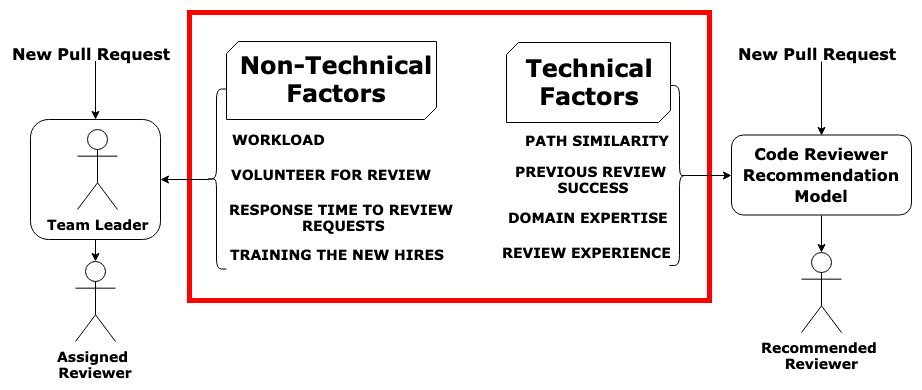
\includegraphics[scale=0.31]{img/final-.png}
    \end{figure}
    \begin{alertblock}{Notice:}
        \begin{itemize}
        \item There exists a discrepancy between real life and algorithm based reviewer selection process.
        \item This discrepancy creates a \textbf{\textit{ground truth problem}} in code reviewer recommendation studies and datasets.
        \end{itemize}
    \end{alertblock}
\end{frame}

\subsection{Ground Truth}
\begin{frame}
\frametitle{\large Ground Truth}

    \begin{block}{Ground Truth:}
    \begin{itemize}
        \item Factual data that has been observed or measured.
        \item If data stands on some assumptions, is subject to opinion, then it cannot be \textbf{ground truth data}.
    \end{itemize}    
    \end{block}
    \pause
    \begin{block}{Ground Truth in Software Engineering:}
    \begin{itemize}
    \item The more human aspects involved, the more tendency to the ground truth problems.
    \item Many fields of empirical software engineering research suffer from the ground truth problem. (i.e. code reviewer recommendation, bug report assignee recommendation, etc.)   
    \end{itemize}    
    \end{block}    
\end{frame}


\begin{frame}
\frametitle{\large Ground Truth}

    \begin{block}{Ground Truth in Code Reviewer Recommendation Studies:}
    \begin{itemize}
        \item Recommendation models rely on the real-life assignments.
        \item These assignments are assumed to be ideal.
        \item Studies in real-life projects show that code reviewers are not usually assigned with the aim of finding the ideal one.
    \end{itemize}    
    \end{block}

\end{frame}

\begin{frame}
\frametitle{\large Reviewer Assignment Scenario in Real Life}
  \begin{figure}
    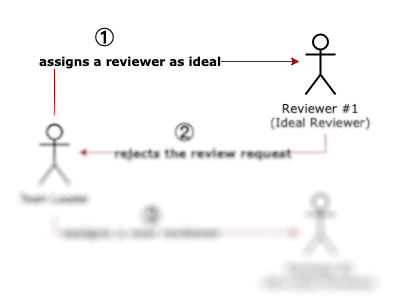
\includegraphics[scale=0.6]{img/gt_1.png}
    %\caption{lion!!}
    \end{figure}

\end{frame}
\begin{frame}
\frametitle{\large Reviewer Assignment Scenario in Real Life}
  \begin{figure}
    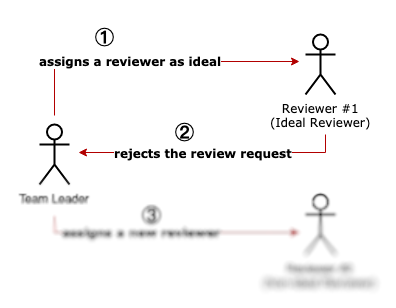
\includegraphics[scale=0.6]{img/gt_2.png}
    %\caption{lion!!}
    \end{figure}

\end{frame}
\begin{frame}
\frametitle{\large Reviewer Assignment Scenario in Real Life}
  \begin{figure}
    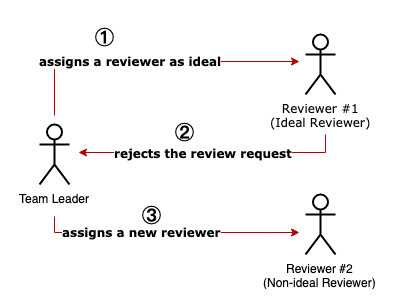
\includegraphics[scale=0.6]{img/gt_3.png}
    %\caption{lion!!}
    \end{figure}

\end{frame}






\begin{frame}{Block, Alert, Example Boxes}

    Define Theorems, draw attention etc. by using boxes.
        
    \begin{block}{Block Title}
        Blocks are colored from Bilkent's color pallette.
    \end{block}
    
    \begin{alertblock}{Alert Block Title}
        Alert block is red.
    \end{alertblock}
    
    \begin{examples}
        This is an example box.. Example boxes are conventionally green.
    \end{examples}
\end{frame}

\subsection{Color Choices of this template}

\begin{frame}{Bilkent Theme}
    Bilkent University's logo have two distinct colors. For more information, see: \url{https://w3.bilkent.edu.tr/www/bilkent-logo/}
    
    \begin{itemize}
        \item Pantone Reflex Blue: \texttt{RGB(0,83,160)}
        \item Flag Red (Alizarin): \texttt{RGB(237,29,36)}
    \end{itemize}
    
    I used darker versions of Flag Red for the structure items such as top and bottom bars.
\end{frame}


\begin{frame}{}

\end{frame}

\section{References}
\begingroup
\Tiny
\begin{frame}[allowframebreaks]
    \frametitle{References}
    \bibliographystyle{apalike}
    \bibliography{bibliography} 
\end{frame}
\endgroup
  %\cite{buyukccakir2018novel}

\end{document}
